% \documentclass[xcolor=svgnames]{beamer}

\documentclass[8pt]{beamer}

\usepackage{amssymb}
\usepackage{textcomp}
\usepackage{wasysym}
\usepackage{listings}
\usepackage{tikz}
\usepackage{adjustbox}
\usepackage{longtable}

\usetheme{default}
\usecolortheme{default}
\useoutertheme{infolines}
\useinnertheme{circles}
\usepackage{outlines}
\usepackage{pdfpages}

%power point font is Verdana but this is probably close enough
\setbeamerfont{title}{family=\fontfamily{phv}\selectfont}
\setbeamerfont{frametitle}{family=\fontfamily{phv}\selectfont}
\setbeamerfont{framesubtitle}{family=\fontfamily{phv}\selectfont}
\usefonttheme{structurebold}
\fontsize{4pt}{7.2}\selectfont

%turn off navigation symbols
\setbeamertemplate{navigation symbols}{}

%define MIT colors
\definecolor{mitmaroon}{RGB}{147,33,53}

%just the page number
\setbeamertemplate{footline}[frame number]{}

\setbeamercolor{frametitle}{fg=mitmaroon,bg=white}
\setbeamercolor{section in head/foot}{bg=white}
\setbeamercolor{author in head/foot}{bg=white}
\setbeamercolor{title}{bg=white,fg=mitmaroon}

\newcommand{\FIX}[1][fixme]{{\color{red}#1}}

\title{MSRI HOPS Redevelopment Review}
\author[Haystack]{J. Barrett, G. Crew, D. Hoak, V. Pfeiffer}
\institute[MIT]{\large MIT Haystack Observatory}
\date{\today}
% \logo{%
%   \vspace{-0.3cm}
%   \includegraphics[width=3cm,keepaspectratio]{./figures/MIT_HO_logo_landscape.png}
%   \hspace{\dimexpr\paperwidth-3cm-10pt}%
% }

\makeatletter
\newcommand\urlfootnote@[1]{\footnote{\url@{#1}}}
\DeclareRobustCommand{\urlfootnote}{\hyper@normalise\urlfootnote@}
\makeatother


%set up the logo (you may need to adjust the coordinates to avoid collisions)
\usepackage{pgf}  
%use the following to put the logo in the top right corner
\logo{\pgfputat{\pgfxy(-1.5,7.6)}{\pgfbox[center,overlay,base]{
\includegraphics[width=2.2cm]{./logo.png}}}}  
%use the following to put the logo in the bottom left corner
%\logo{\pgfputat{\pgfxy(-10.8,0.0)}{\pgfbox[center,overlay,base]{
\includegraphics[width=2.2cm]{./logo.png}}}}  

%the following latex nonsense keeps the logo from getting clipped by frame titles
\makeatletter
\setbeamertemplate{frametitle}
{
  \ifbeamercolorempty[bg]{frametitle}{}{\nointerlineskip}%
  \@tempdima=\textwidth%
  \advance\@tempdima by\beamer@leftmargin%
  \advance\@tempdima by\beamer@rightmargin%
  \pgfsetfillopacity{0.0}       %<------ fix filling opacity
  \begin{beamercolorbox}[sep=0.3cm,left,wd=\the\@tempdima]{frametitle}
    \usebeamerfont{frametitle}%
    \vbox{}\vskip-1ex%
    \if@tempswa\else\csname beamer@fteleft\endcsname\fi%
    \strut\pgfsetfillopacity{1}\insertframetitle\strut\par%  <---- text opacity
    {%
      \ifx\insertframesubtitle\@empty%
      \else%
      {\usebeamerfont{framesubtitle}\usebeamercolor[fg]{framesubtitle}\insertframesubtitle\strut\par}%
      \fi
    }%
    \vskip-1ex%
    \if@tempswa\else\vskip-.3cm\fi%
  \end{beamercolorbox}%
}
\makeatother
 


\begin{document}

\renewcommand{\outlinei}{enumerate}
\renewcommand{\outlineii}{enumerate}
\renewcommand{\outlineiii}{itemize}


\begin{frame}
\titlepage
\end{frame}


% \begin{frame}{Guidance given by J.S.}

% TODO - remove this slide (just for reference)
% \begin{outline}
%   \1 Requirements that the project is working to (including identification of key interfaces), rationale for those requirements, and how they support the main project purpose
%   \1 Specific development plan and design approach (i.e. How have initial design decisions been made? With what assumptions? What design iterations are you planning? What is the current state / maturity of the design?)
%   \1 How development plan addresses requirements
%   \1 Schedule
%   \1 Budget, esp. comparison with budget originally proposed (hopefully equal to or less than)
%   \1 Risks and risk mitigation plans 
% \end{outline}

% \end{frame}

\begin{frame}{Outline}
    \begin{outline}
        \1 Snapshot \& Background
        \1 Scope, Requirements, and Assumptions
        \1 Software architecture and identified interfaces
        \1 Development plan
        \1 Current design state
        \1 Schedule
        \1 Risks/Mitigation
    \end{outline}
\end{frame}


% Add a high level schedule of the program at the start of the slides:
%  - people will come in with preconceptions; explicitly say we're doing exactly what we promised, on track and schedule
%  - Add a chart (few bars) to show where we are in the project and where this review fits in
% Is there anyone in the audience who might not know what HOPS does?
%  - add a couple of sentences to explain the workflow of fringeing data
%  - problem of defining where HOPS starts and ends; it can do more than postprocessing
%  - backend is important; say we don't plan to do more than what HOPS currently does?
%  - goal is to revise HOPS so it is easier to be extensible (describe this as an architectural change?)
%  - data summarization software (A-tools) are still used & need to be made more accessible (python wrappers)
%  - A-file tools have hooks back into the fourfit path

% Maybe mention A-tools in the background/scope, and the functionality they provide

\begin{frame}{Quick Snapshot}
\centering
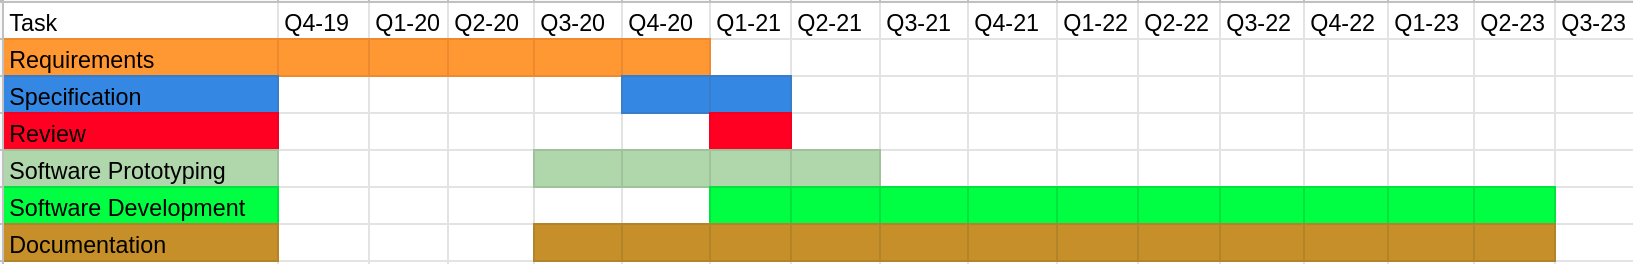
\includegraphics[width=\textwidth]{snapshot-schedule.png}
\begin{outline}
    \1 Delayed start, but original schedule had plenty of margin
    \1 Largely on track/schedule - dev. plan document under revision
    \1 Software development/prototyping stage has started and in progress.
\end{outline}
    
\end{frame}

\begin{frame}{Background}
    
    \begin{outline}
      \1 HOPS has a multi-decade history as a post-processing/analysis package and as such has evolved gradually over time.
        \2 Current C-code was written in the early 90’s by Colin Lonsdale, Roger Cappallo and Cris Niell. The basic algorithms were adopted from FRNGE, by Alan Rogers in the late 70's
        \2 Efforts in the 00's with tools to optimize SNR and in response to software correlators such as DiFX.
        \2 For the 2017 EHT campaign, HOPS was augmented with python-based packages. HOPS performed well when measuring delays and correlation coefficients (compared to AIPS, CASA)
      \1 Primary component is the fringe-fitting software \textit{fourfit}.
      \1 Also includes data summarization software (alist/aedit) -- provide diagnostics for debugging correlation and evaluating data quality.
      \1 HOPS has reached the limits of what can be fixed with ``bandaids"
      \1 Due to current architecture, HOPS (and \textit{fourfit}) is difficult to extend/modify
    \end{outline}
    
\end{frame}

\begin{frame}{Assumptions: Use-case model}
% slide 6 & 7: avoid "somewhat" (too vague) - don't use vague language ("four" instead of "a few", where possible)
%  - "three major monolithic applications and several minor ones"

\begin{outline}
  \1 Assumed that general use-cases for the new HOPS software package are expected to follow the existing use model and be a combination of processes consisting of:
  \2 Import/Export of data from a software correlator (DiFX).
  \2 Data flagging/removal of corrupted visibilities in time/frequency.
  \2 Calibration and phase/amplitude correction of data, as well as other manipulation (summing over polarization products, etc.)
  \2 Fringe-fitting (solving for residual phase/delay w.r.t to correlator model) on either a per-baseline or global basis.
  \2 Data quality analysis and visualization on a per-scan and per-experiment basis.
  \2 Data export to archival and/or imaging formats (example: HDF5/UVFITS).
\end{outline}
    
\end{frame}

\begin{frame}{Further Assumptions}

% \FIX[DRAFT SLIDE]

\begin{outline}
    \1 Fine grained details may not be explicitly covered in requirements. Some assumptions are baked into the requirements, examples:
        \2 HOPS4 will accept DiFX correlator input (including VEX at current v1.5.1) 
        \2 ngEHT data format will resemble EHT data, except for more stations/baselines/sub-bands.
        \2 General computational performance of \textit{fourfit} in HOPS3 was acceptable for EHT (with SPMD parallelization).
        \2 General software run-time environments will be similar to HOPS3 (unix like)
    \1 Some details are not known, example:
        \2 Memory requirements of ngEHT data sets.
        \2 Possible unspecified future use-cases
    \1 These assumptions entail risks - the assumptions may be wrong, and the code may require modification to meet them -- can discuss in risks section.
\end{outline}

\end{frame}



\begin{frame}{Scope and Requirements}

% slide 5: MH: dynamic memory allocation "induces a limit" -> "imposes a limit"
% maybe rename slide to suggest these are fixes?
% detailed requirements in a documents -> say which documents

\begin{outline}
    \1 The overarching goal of this project is to upgrade/replace the existing HOPS software with a modern and extensible version not subject to the limitations of the old package while still maintaining the existing capabilities.
    \1 Generally speaking the limitations we aim to eliminate are both technical and
    practical in nature:
        \2 Technical:
            \3 Limited or no ability for dynamic memory allocation, which imposes a limit on the number of stations, APs, and sub-bands (channels).
            \3 Fully complex (amplitude and phase) band-pass corrections are not possible (only phase/delay corrections).
            \3 Only a single per-scan/baseline fringe-finding algorithm is available 
            \3 Currently no support for multi-processing, apart from SPMD
        \2 Practical:
            \3 Control file syntax is arcane, plotting and results are not decoupled
            \3 Custom data treatment (e.g. band-pass correction) is limited to that which is allowed by the control file parameters or ad-hoc phase files (i.e. no easy way to inject custom code, whether that be compiled-in or scripted).
            \3 File and data formats (Mk4-types) which are restrictive and not easily modified, and tightly coupled to code.
            \3 Reliance on out-dated/unsupported libraries (e.g. PGPLOT).
    \1 Further details in the distributed requirements document (v1.0).
\end{outline}

\end{frame}

\begin{frame}{Software Architecture}

% slide 6 & 7: avoid "somewhat" (too vague) - don't use vague language ("four" instead of "a few", where possible)
%  - "three major monolithic applications and several minor ones"

\begin{outline}
  \1 The previous/existing HOPS architecture is composed of three major monolithic applications (fourfit, alist, aedit) and several minor ones (cofit, average, fourmer, search, etc).
  \1 Software is supported by four low-level libraries (mkutil, dfio, afio, vex)
  \1 New architecture is an object oriented component-based design to be composed of a set of loosely coupled task-specific libraries along with a similar set of (extensible) applications.
  \1 The new architecture will also support extension of the library/application code in two ways:
    \2 Developer (compile-time) extensions to data-manipulation will be added as needed as new derived classes of a basic set of 'data operators'. These can then be configured and inserted into the application control flow at run time.
    \2 User (run-time) extensions will be supported by a python plug-in interface, consisting of bindings to the in-memory data containers and operators, and a series of hooks (at specific points) in the application code where a user-script can be injected.
    \1 The choice of C++ as the development language for the new libraries is discussed in the specifications document (v1.0).
\end{outline}

\end{frame}

\begin{frame}{Software Architecture (Internal dependencies)}

% page 8: I (DH) like this slide, I think the arrows are very sensible
%  - Is the audience familiar with UML diagrams? (this is not a real UML diagram)
%  - add some text to explain the slide
%  - Colin: what about C++? will anyone ask why? "choice of language is discussed in specifications document"

\centering
    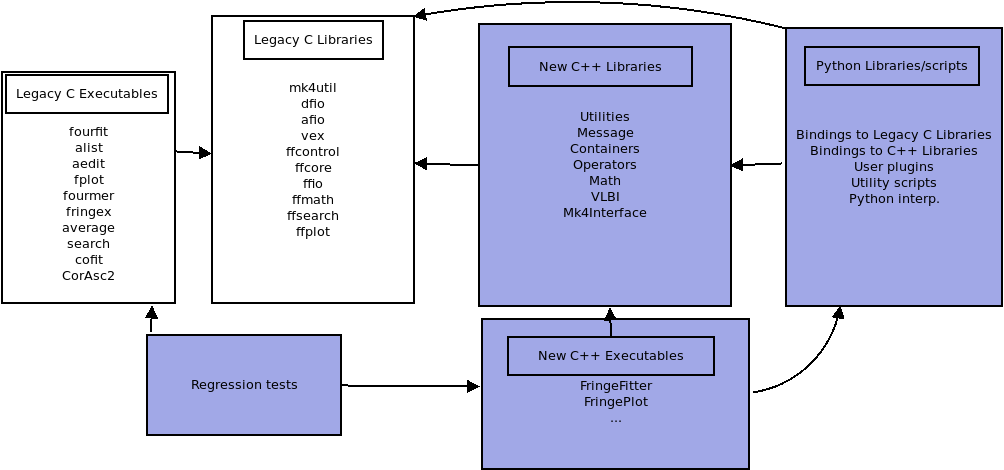
\includegraphics[width=\textwidth]{arch_overview.png}
    \vspace{0.75cm} \\
    Dependency relationships of the main internal software components. Shaded boxes are new components of this project. Arrows indicate direction of dependence (point from child to parent).
\end{frame}

\begin{frame}{Software Architecture (Libraries)}

\begin{outline}
  \1 Legacy c-libraries (made available for re-use and backwards compatibility)
    \2 dfio - I/O for MK4 data types
    \2 mk4util - utility library for MK4 data types
    \2 afio - I/O library for alist manipulation
    \2 vex - vex parsing library
    \2 fourfit specific libraries (maintained to provide legacy-fourfit application):
        \3 ffcontrol - parse old-style fourfit control files 
        \3 ffcore - core parameter structures
        \3 ffio - output for fringe file data
        \3 ffmath - trivial math routines used by fourfit
        \3 ffplot - fringe-plot generation library 
        \3 ffsearch - core fringe-search algorithm library (grid-search)
\1 New C++ libraries* 
    \2 Containers - In-memory data containers of visibility and meta-data and native format disk I/O
    \2 Utilities - Commonly used utilities (e.g. date handling, profile timers, object toolboxes, etc.)
    \2 Math - Math routines: FFTW, minimizers, interface to optional 3rd-party math libraries
    \2 Message - Controls the topic and verbosity level of application messages/logs to user
    \2 MK4Interface - Allows for import/export to legacy MK4-types for testing and backwards compatibility
    \2 Operators - Base classes for data manipulation, and generic operations (array reduction, transposition, FFT, etc.)
    \2 VLBI - VLBI task-specific operators (e.g. band-pass correction, per-channel phase offsets, etc.)
    \2 Bindings - Python interface to C++ data containers and operators. Allows for Python script configuration of data operators at initialization, and user-defined direct manipulation of data at pre-defined hooks.
\end{outline}

* current working names
\end{frame}

\begin{frame}{Software Architecture (Applications)}

% slide 9/10: watch tense, say "will be reworked"; "possible" is too vague, is it an option if time permits? (maybe an option to be descoped?)
% philosophy: how about "current functionality will be preserved to meet new requirements, and enhance capabilities for expansion"
%  - scope of python interface is TBD (last bullet on slide 9)

% slide 11: "possibilities": upcoming trades between X/Y; don't say "we might do this we might do that" 
%  - "need to be" -> "will be"; say what you won't do
%  - architecture to support optimization of global vs single-shot fitter; architecture to allow users to define precise fitting methods

HOPS4 will maintain functionality that replicates the following HOPS3 applications.
\begin{outline}
  \1 essential tools:
  \2 fourfit - (fringe fitter) - will be completely overhauled
  \2 alist - (fringes $\rightarrow$ .alist files) - support version 6
  \2 aedit - (manipulator of .alist files) - will be enhanced, with a Python interface
  \1 additional tools:
  \2 average - (slicer/recombiner of alists) - will be reworked
  \2 cofit - (coherence estimator) - will be reworked/replaced
  \2 fourmer - (fringe joiner) - will be reworked
  \2 fplot - (fringe display tool) - will be reworked
  \2 search - (for marginal fringes) - will be reworked
  \2 CorAsc2 - (data dumper) - used for mk4 regression
  \1 additional scripting
\end{outline}
Again, the philosophy is to preserve the current functionality, refactor the back-end to meet new requirements, and significantly enhance capabilities for expansion.
%to not break things that currently exist and significantly enhance the range and ease of use for the toolset.
\end{frame}

\begin{frame}{Simplified Fringe Fitting Architecture}
\centering


\begin{columns}[T]
  \centering
    \begin{column}{.5\textwidth}
    \centering
    \begin{minipage}{5cm}
    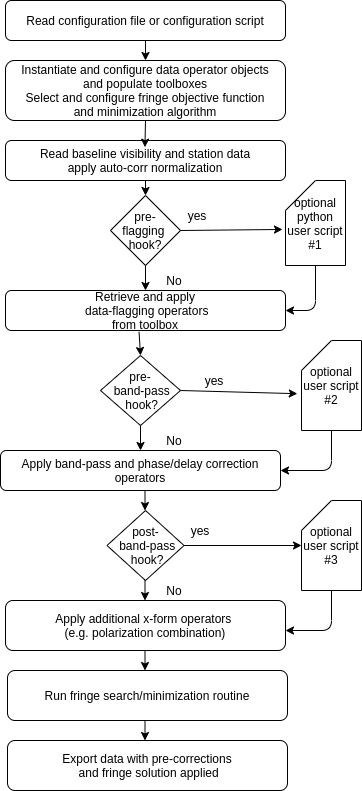
\includegraphics[width=0.7\textwidth]{./example-single-baseline-fringe-fitter.png}
    \end{minipage}
    \end{column}
  \begin{column}{.6\textwidth}
  \centering
  \hspace{-3cm}
  \begin{minipage}{8cm}
\vspace{1cm}
Example of simplified fringe-fitter control flow.
    \begin{outline}
        \1 Architecture to support single-baseline or global fringe fitter built from common library components.
        \1 Data containers and data operators will be as decoupled as possible.
        \1 Data operators will be configured/instantiated and then inserted into ordered slots
        \1 Data operator requirements on the data/meta-data will be specified via a schema for key:value retrieval through common interface to keep data contents from affecting the interface. Example: apply phase offset to channel.
        \1 Provide hooks to insert user python code (direct access to data and instantiated data operators) -- important for specific tasks beyond immediate scope of this project (e.g. application of antenna gain cal.)
        \1 Python interface to data containers is TBD. Trade-offs between ease of use
        and performance (data-copy) need to be evaluated.
    \end{outline}
    \end{minipage}
    \end{column}
  \end{columns}
  
\end{frame}

\begin{frame}{Identified Interfaces}
    \begin{outline}
    \1 Data movement interfaces:
        \2 Data I/O and conversion from correlator DiFX format to HOPS native format.
        \2 HOPS native format to disk I/O for persistence.
        \2 Import/Export of legacy MK4-types to HOPS native format.  
        \2 Export of HOPS native format to external archive format (e.g. HDF5/UVFITS).
        \2 Reduction of fringe-files to data summary format (alist).
    \1 User interfaces:
        \2 Configuration of fringe-fitting routine (requires python interp. and bindings).
        \2 Custom user data-manipulation scripts (requires python bindings). Note this also allows custom data-export routines various points in the code.
        \2 User interaction with plotting and data inspection utilities.
    \end{outline}
\end{frame}

\begin{frame}{Interfaces cont.}
\begin{outline}
    \1 Python bindings to executable C/C++ objects/modules in Python (SWIG/pybind11)
    \1 Python bindings to in-memory data objects to python wrappers (SWIG/pybind11)
    \1 Conversion/interpretation of legacy control-file format
    \1 Linking to external dependencies:
        \2 FFTW3 (with fallback to native library)
        \2 SWIG/pybind11 is only required for developer/maintainers
        \2 Doxygen/Sphinx for developer/maintainers
        \2 Minimal set of Python required (numpy, matplotlib, ...TBD)
\end{outline}
\end{frame}

\begin{frame}{Development Process}
% slide 21: don't need to describe the test plan (takes time to read); do we need to write this in terms of developers?
    \begin{outline}
        \1 Agile Development
        \1 Feature additions progress through 5 stages:
            \2 concept - what does this feature need to do?
            \2 prototype implementation - initial code implementation
            \2 integration test - test executable, does it function as needed?
            \2 performance evaluation - is feature resource use appropriate?
            \2 incorporation - merge back into code-base, put into use
            \2 regression - demonstrate that new code matches (or improves on) performance and results of HOPS3
        \1 Weekly status meetings, otherwise meet when necessary
        \1 Internal due dates for code changes (weekly or biweekly, depending on feature).
        \1 Daily testing with CI server, initially to ensure functioning build system, progressing to include full regression and integration tests.
        \1 Automatic doxygen documentation generation
    \end{outline}
\end{frame}

\begin{frame}{Development Plan}

% slide 14: It's possible the development plan needs harder boundaries of scope: will accomplish, items for which we might have marginal resource, and desires
% Colin: HOPS has a facility to examine data very closely - will be retained? (not clear if audience is aware - maybe needs to be advertised)
% slide 14: prioritization of build-out of software
%  - core components
%  - base classes, operators, utilities
%  - independent components
% "we will take a hierarchical approach & will build things in order of importance"?
% remember, saying something is important is not the same as we'll do it for sure

    \begin{outline}
    \1 Iterative process taking a hierarchical approach -- build base components first, fill in details and specialized extensions later
    \1 Code experimentation/testing is key to locating deficiencies in the design as it progresses. Fail fast/early approach
    \1 Order in which components are developed/introduced depends on:
    \2 Is it a core component of basic infrastructure? -- e.g. build system, messaging and logging utils etc.
    \2 Is it low-level code upon which many libraries/components depend -- e.g base classes for data structures, data operators, and utilities, testing infrastructure
    \2 Is it nearly independent from other components (no new or only well established deps.) -- e.g. python plotting routines, break-out of HOPS3 code into shared libraries
    \end{outline}
\end{frame}
    
\begin{frame}{Development Plan (component build-out order)}

% slide 15: make things verbs: write build system, import HOPS3 libraries, populate data operators, etc

    \begin{outline}
    \1 Write the build system and testing infrastructure
    \1 Import HOPS3 libraries and 'frozen' executables
    \1 Implement data containers for visibility and meta-data
    \1 Convert libraries/executables to import/export visibility and meta-data (DiFX, MK4 formats)
    \1 Populate the basic data operators (FFT, sum/reduction, functor-broadcast)
    \1 Populate the minimally necessary (VLBI specific) data operators (e.g. normalization, manual phase-cal, delay-cal) to mimic existing HOPS3 fourfit functionality
    \1 Implement python bindings to data containers and data operators in parallel with the above.
    \end{outline}
\end{frame}

\begin{frame}{Development Plan cont.}

% slide 16: applicable? if we have time? how to evaluate. new framework will allow, but depends on time / option to descope
%  - fourth bullet "implement a global fringe algorithm"
%  - bullet on global fringeing, alternative fringe fitting

\begin{outline}
    \1 Implement minimally-viable grid-search single-baseline fringe-fitter 
    \1 Continue build-out/reuse of rest of current existing fourfit control-file features as data operators
    \1 Augment with new data operators (fully complex band-pass correction, condition based data flagging, etc.)
    \1 Implement data-inspection (plotting, alist/aedit) and export tools
    \1 Implement a global fringe fitting algorithm as an alternative to baseline-based, either as a configurable-option or separate executable (precise algorithm not specified; option to descope)
    \1 Augment data operators with SIMD parallelism (option to de-scope)
    \1 Implement distributed (OpenMPI) fringe-fitter (option to de-scope)
    \end{outline}
\end{frame}

\begin{frame}{Current Design State}

% slide 17: when will it be frozen?  likely to patch HOPS3 up until delivery of HOPS4
%  - "will be frozen prior to delivery to HOPS4", maintained for ~4 years (TDB)
%  - simplify language, make declarative, don't give so much information
%  - embryonic -> "HOPS4 development has started, key technologies have been demonstrated"
%  - not rearranging furniture -> refactoring code into task-specific libraries

    \begin{outline}
    \1 HOPS3 is operational, will be maintained and patched until delivery of HOPS4.
        \2 Maintained in SVN; will be "frozen" prior to delivery of HOPS4. Frozen copy will be maintained at Haystack for 4 years (TBD).
        \2 The subset of HOPS3 libraries/executables to be retained in HOPS4 will be migrated to the new GIT repository (partially complete)
    \1 HOPS4 development has started and key technologies have been demonstrated
        \2 basic utilities and data container/operator prototypes exist
        \2 Mk4-type import/export code in progress 
        \2 Builds (mostly) with both Autotools and CMake
        \2 Organizing bases classes of code in task-specific libraries
        \2 Development allows re-use of HOPS3 code in decoupled manner (e.g. MK4Interface makes use of dfio and (new) container library but there is no direct link between the two)
        \2 SWIG build infrastructure has been prototyped, pybind11 will also be explored.
        \2 Fringe-plot code starting to be prototyped in python/matplotlib.
    \end{outline}
\end{frame}

\begin{frame}{Prototyping Data Container Class Structure}

\begin{columns}[T]
  \centering
    \begin{column}{.65\textwidth}
    \centering
    \begin{minipage}{9cm}
    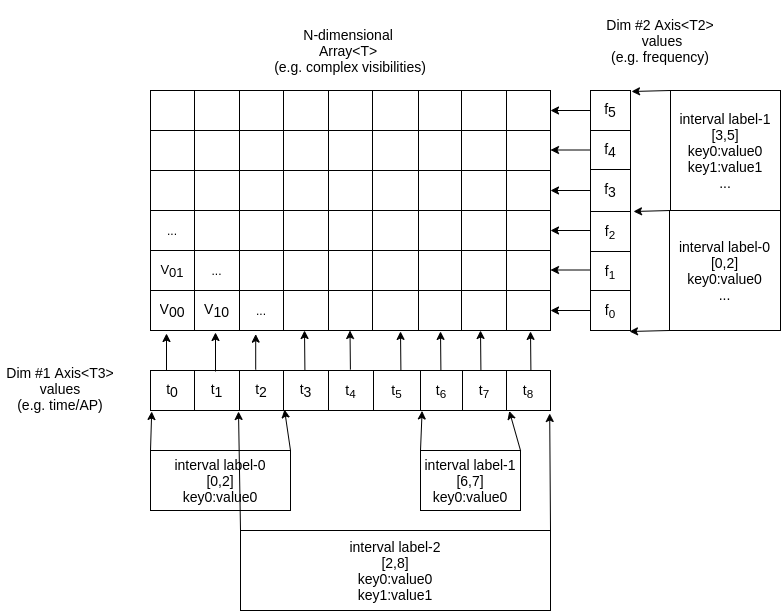
\includegraphics[width=\textwidth]{data-container-baseline.png}
    \end{minipage}
    \end{column}
    \hspace{0.5cm}
  \begin{column}{.2\textwidth}
  \centering
  \begin{minipage}{3cm}
  \vspace{1.5cm}
    \begin{outline}
    \1 Graphical representation current data container prototype code
    \1 ND-array template class with type and rank parameters + STL-style iterators
    \1 Axes templated on coordinate type
    \1 Intervals of array can be labeled with type-agnostic key:value pairs for
    data selection
    \end{outline}
    \end{minipage}
    \end{column}
  \end{columns}

% slide 18: make title/bullets specific that this is an example of prototyped data container structure (new, existing code)

% \FIX[Need to add some descriptive text to this slide: title/bullets to clarify this is an example of a prototyped data container structure (new, existing code)]

\end{frame}

% slide 19: first bullet point, PGPLOT has not been supported, will not be included as required package


\begin{frame}{Prototyping Plotting Toolkit}
\begin{columns}
\column{0.5\textwidth}
\begin{outline}
    \1 PGPLOT is no longer supported and will not be included in the required dependencies for HOPS4
    \1 Need to build new plotting functionality to distribute with HOPS4:
    %    \2 Difficulty to include as a required package has reached a tipping point 
    \2 Separate analysis results from plotting (these are tightly coupled in HOPS3)
    \2 Write new plotting routines with Python/NumPy/Matplotlib
    \2 Include support for arbitrary plotting tools, hooks for other packages
    \2 Develop interactive tools to allow users to reformat plots, explore and select data, flag datapoints, etc.
\end{outline}
\column{0.5\textwidth}
\centering
\includegraphics[width=\textwidth]{matplotlib_fringe_plot.pdf}
Example of a fringe plot made with Matplotlib
\end{columns}
\end{frame}



\begin{frame}{Testing}

% slide 20: testing step? add step 6 for regression
%  - remove "as appropriate"



    \begin{outline}
        \1 Unit/Integration - Code changes and new functions/modules will be delivered with appropriate units tests
        \1 Performance analysis - A profiling tool will be used to compare the time/memory use of computations in HOPS3 with HOPS4, to identify bottlenecks.
        \1 Manual - Document tests to verify human-in-the-loop functionality (e.g. interactive tools)
        \1 Regression - Write tests that compare quantitative results of the new code with known results (e.g. from HOPS3) with captured data.
        \1 CI - A continuous integration server will be configured using Github Actions or be made compatible with our existing automated testing scripts.
        \1 Component - External dependencies will be tested to ensure continuous compatibility with HOPS4.
        \1 Oracle - Where appropriate, HOPS3 will be used as a test oracle for HOPS4 comparison.
    \end{outline}
    
\end{frame}


\begin{frame}{Provisional Schedule}
% 22: reformat plot? or, take out timeline bars, just use begin/end dates
%  - say we already sent around the schedule, add figure to backup slides
%  - largely indicated by -> determined by
%  - most of these tasks proceed asynchronously; tasks can move around without effecting others; interdependency between tasks is minimal; progress checkpoints correspond to release of following executables

    \centering
    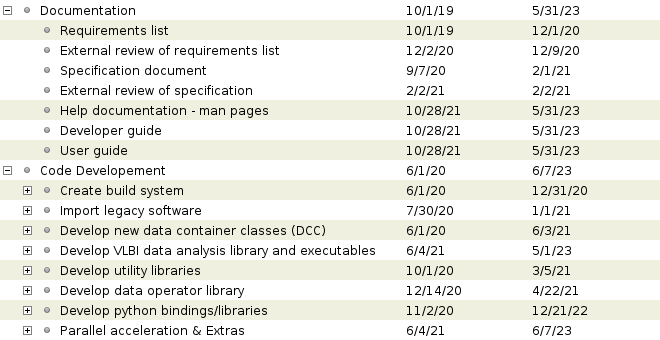
\includegraphics[width=0.75\textwidth]{sched.png}
    \begin{outline}
    \1 Status reports will indicate the readiness of the following:
        \2 Mk4-types import/export utility
        \2 DiFX import utility
        \2 Minimally viable single-baseline fringe fitter $\rightarrow$ complete fringe fitter equivalent to HOPS3 fourfit
        \2 Data reduction utilities (alist, aedit, fringe plot)
        \2 augmented single-baseline fringe fitter 
        \2 Data export utilities (e.g HDF5).
        \2 global fringe fitter
    \1 Tasks proceed largely asynchronously
        \2 Can move some tasks in the schedule without affecting others
        \2 Interdependency between tasks varies - does not waterfall
    \end{outline}
\end{frame}

\begin{frame}{Budget}

% slide 23: budget is adequate?  comment on feasibility of the budget
%  - descope plan: will meet requirements, but may descope additional features
%  - define what it means to be pragmatic about project scope
%  - budget is expected to be adequate, here's what we'll do if it's 
%  - explicitly say we will descope capability if becomes pressured
%  - resources are sufficient to complete coding for A, B, C modules
%  - clear idea of what we're confident we can do, what we'll do if we have time, what we'll add if we have time leftover
%  - list of core capabilities, descope-able capabilities, and then wish list
%  - Again, development plan scope: sufficient margins to accomplish the following, best effort on the following as resources allow (will install hooks to enable external development), currently unlikely to accomplish
%  - HOPS development doesn't end with the MSRI; ngEHT may have resources to extend the project
%  - State that our goal is to refactor HOPS and put it in a position where it can be extended without having to rewrite core libraries


Comments:
\begin{outline}
    \1 Budget is adequate: sufficient margins to complete coding though rebuilt fringe-fitter and utilities:
        \2 DiFX/Mk4 data import/export
        \2 fourfit equivalent with new architecture
        \2 aedit
        \2 alist
        \2 data export
    \1 At a minimum HOPS4 will be capable of everything which HOP3 can do now, but be more easily extended by users, and not suffer from artificial bandwidth/AP/station limitations. Goal is to refactor HOPS and position it to be extendable without requiring changes to core libraries.
    \1 If resources are pressured, will apply best effort to:
        \2 Implementing prioritized critical features (e.g. solving for stationized band-pass correction vs. global fringe fitting algorithm)
        \2 Option to de-scope some capabilities (e.g. SIMD or OpenMPI paralleliztaion).
\end{outline}

\end{frame}



% risks to keep:
% bug in commit: discovered late in process, funding for ongoing support

% another risk: ngEHT has not defined data requirements
%  - ngEHT requirements may change (data types, format, fringeing needs?)
%  - when it's defined may not be compatible with structure we've developed
%  - assumptions slide at the beginning: details of what we assume they expect us to do in areas where requirements are ill-defined
%  - ngEHT has not defined memory needs (& here's all the ways we think this could get us into trouble

% Standard framework: define risk (strut is found to be weak), define cost (bridge falls down), define mitigation (add strength, costs $$), identify the decision point on mitigation (when do we spend money).
% Example: risk is bug discovered after delivery with no resources to fix it, cost is committing resources for testing

% Add decision points to mitigation section/column
% Note that our risks are primarily schedule risks, for this project

% Look at risk register examples. Organized as: topic, impact if realized, current practices, additional measures (e.g. will cost additional resources)

% Items that are common to all projects should not be included as risks (like personnel)

% Mention pportunities to descope: are there functionalities that we don't need to maintain?
%  - don't mention, might get us in trouble with geodesy

% Include an issues & concerns slide (not risks): when we're done, ppl might be unhappy with the speed
%  - by some metric, code is too slow, need to rewrite in C++, when will we need to decide

% dependencies moved to issues/concerns
% under-perform -> doesn't meet requirements

% Our requirements are incomplete at low levels
% We are a small project, don't have resources to define low-level requirements, introduces some uncertainty, address with sufficient margins and descope plan


% Todo: Join monthly MSRI risk meeting (tomorrow's meeting is for risk, I think).

% One approach to avoid further bureaucracy: our risk register is internal, will forward to project risks that should be tracked at the project level (source of friction in the past?)

\begin{frame}{Risk Management}

\begin{outline}
    \1 Maintain internal prioritized risk-action list, touched on in weekly meetings; any team member can raise issue for review.
    \1 Since this is a software project, our risks are primarily \emph{schedule} risks (i.e. developers will have to spend time mitigating them). The costs to mitigate are primarily budgetary (\$\$ for developers' time).
    \2 Issues which rise beyond internal project scope will be raised to monthly ngEHT risk meeting.
    \2 Minor software risks (bugs) are mitigated by testing and profiling code early, iterative development
    \1 We don't include generic problems that are common to all projects as risks (loss of personnel, dependency no longer supported, etc).
    \1 Current hi-level risks:
        \2 Requirements are incomplete due to unanticipated ngEHT needs or failure of assumptions.
        \2 Unexpected bug or structural deficit in new code (amplified if discovered late in process).
\end{outline}

\end{frame}


% \begin{frame}{Issues \& Concerns}
% \begin{small}
% %\newcolumntype{R}{>{\raggedright\arraybackslash}p{4cm}}
% %\begin{table}
%     \begin{longtable}{p{4cm} c c p{4.5cm}}
%         & \multicolumn{2}{c}{\footnotesize L=Low, M=Medium,} \\
%         & \multicolumn{2}{c}{\footnotesize H=High} \\
%         \bf Risk & \bf Likelihood & \bf Cost & \bf Mitigation \\

%         \hline
            
%         New automation tool & M & L & Fall back on configuring existing test scripts with the Github repo \\ \hline
            
%         Memory leak	& L	& L	& Use a performance analysis tool regularly \\ \hline
            
%         Bugs introduced in a commit & L & L & Use continuous integration \& nightly jobs to check for errors \\ \hline
            
%         New container architecture & M & M & Test data containers early in the project and check at regular intervals \\ \hline
            
%         Change in requirements & L & L & Use the Agile development process \\ \hline
            
%         Change in personnel & L & M & Train the new personnel and divide up the work in ways that they can handle \\ \hline
            
%         New C++ language use & L & M & Fall back to just using C for the new data container types or use another language like Rust \\ \hline
            
%         Dependency is deprecated & L & M & Replace with a modern one. (Our goal for HOPS4 is to have minimal dependencies.)\\ \hline
%     \end{longtable}
% \end{small}
% \end{frame}

% \begin{frame}{Issues \& Concerns II}
% \begin{small}
%     \begin{longtable}{p{4cm} c c p{4.5cm}}
%         \hline           
%         New data types require support and/or don't cover all future data-needs & M & M & Maintainers can modify code or add entirely new data-types, also and option to export data immediately post-correlation to an open format (such as HDF5) can be made available \\ \hline


%         Loss of personnel & L & H & Manage code via version control and update documentation periodically to ensure knowledge transfer \\ \hline
            
%         Native math libraries under-perform & L & M & Profile code to detect bottle-necks when under development, fall-back to 3rd party libraries (fftw3, GSL) if effort too high \\ \hline
            
%         Community VEX standard shifts from v1.5.1 to v2.0  & * & * & After correlation, store all relevant vex data in community supported open-format (xml, json) - requires 3rd party library \\ \hline
        
%         Python plugin-architecture is too slow & M & M & Direct access to underlying data (rather than copy) is preferred. Intensive python analysis scripts can be re-written as c++ classes. Python will only be used as a wrapper. \\ \hline
            
%         ngEHT data-sets require more memory than available on typical commodity computer & M & M & Use special hardware instances (e.g AWS EC2 high-mem). Or write OpenMPI version of application capable of distributing data-set over multiple computers \\ \hline
        
%     \end{longtable}
% \end{small}
% \end{frame}

% \begin{frame}{Issues \& Concerns III}
% \begin{small}
%     \begin{longtable}{p{4cm} c c p{4.5cm}}
%         \hline
            
%         ngEHT computational load is too high for typical commodity computer & M & M & Fringe-fitting is embarrassingly parallel, so run different data-sets on multiple-machines at once. Alternatively, exploit specialized hardware extensions (SIMD, OpenCL). \\ \hline
            
%         Old/legacy data analysis no longer possible or easy to perform in new HOPS & L & L & While no longer actively developed, the old HOPS software will still be available and maintained in its current form. Regressions tests should catch significant deviations from old code. \\ \hline

%     \end{longtable}
%     %\caption{Risk assessment matrix}
%     \label{tab:risk}
% %\end{table}
% \end{small}
% %*topic for discussion
% \end{frame}

\begin{frame}{Thanks for listening!}
    \centering
    Questions/Comments/Follow-up report?
\end{frame}

\begin{frame}{Backup (Schedule)}
\centering
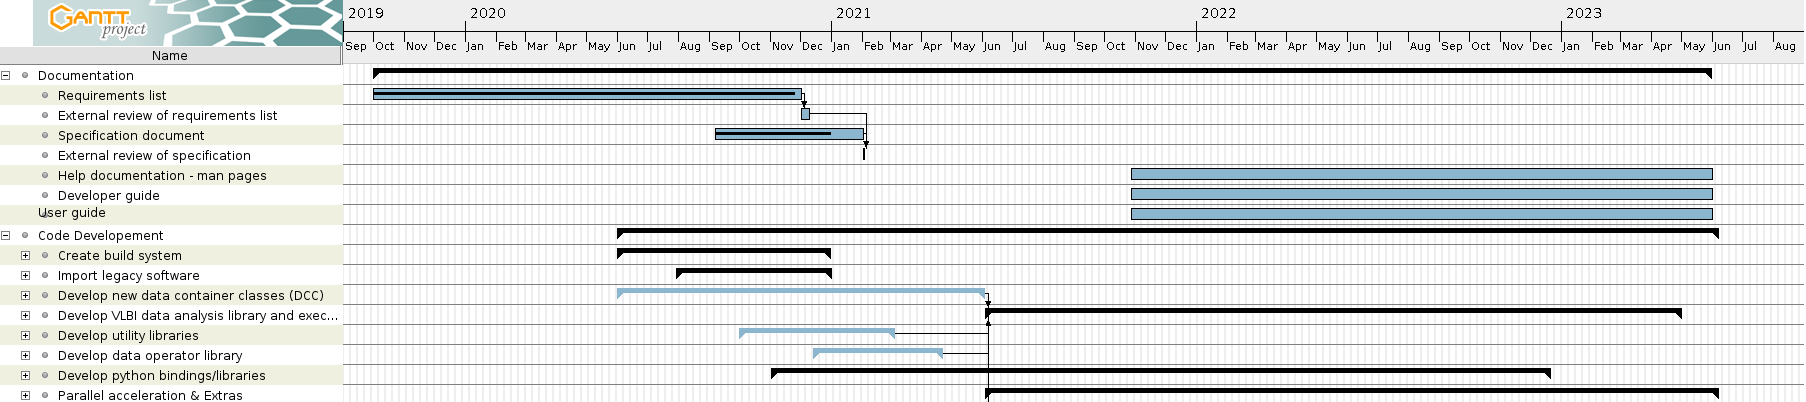
\includegraphics[width=\textwidth]{MSRI-HOPS-2021-3.png}
\end{frame}

\begin{frame}{Risk Details - I}
  
 \begin{outline}
        \1 Incomplete requirements:
            \2 Description: The requirement set is incomplete and doesn't cover a critical item needed for ngEHT data analysis or use cases.
            \2 Preventative Mitigation: Keep code as modular as possible, so extensions/restructuring are limited in scope.
            \2 Cost if realized: Code needs to be extended, adapted or redesigned to cover the necessary use case. Other features of project may need to be descoped to free up resources, or other alternatives considered (adoption of 3rd party libraries).
            \2 Specific example(s): 
            \3 ngEHT correlator output data format/content is not similar to the EHT and data structures have to be redesigned.
            \3 ngEHT data sets are too large to fit in commodity computer memory.
    \end{outline}
    
\end{frame}

\begin{frame}{Risk Details - II}
    
    \begin{outline}
            \1 Unexpected bug/deficit:
            \2 Description: A software deficiency or bug is discovered which significant requires developer resources in order to correct.
            \2 Cost if realized: Developer time must be reallocated to correct issue -- (same as above).
            \2 Preventative Mitigation: Continuous testing/comparison to working (HOPS3) code and performance evaluation of features as they are completed. Issue a beta release of software to downstream users before project completes. 
            \2 Specific example:
                \3 Downstream users find that Python plugin interface is too slow.
    \end{outline}
    
\end{frame}

\end{document}


